\hoofdstuk{Main research }
This chapter will define the main research process. 

\paragraaf{Introduction}
The goal of the main research is get a hands on with the framework. Does it have the features Lunatech wants? Is it suitable for adoption by lunatech? In other words: "\emph{Is Titanium viable for commerical useage?}"

%so what is viable?
\paragraaf{Defining viable}
To determine if a cross-platform mobile application development solution is considered viable for commercial usage a set of criteria has been provided by Lunatech.
\begin{itemize}
	\item \emph{Extensibility}\\
	How new features can be added to the existing framework.
	\item \emph{Maturity}\\ 
	Maturity of underlying code. & implementation of features.
	\item \emph{Documentation}\\
	How existensive and accessible the documentation is.
\end{itemize}

Extensibility
When the developer wants to implement a custom feature in the solution, the interfacing api should be easy to understand and use

Maturity
The code underneath the API should be free from bugs' and programming errors.
Indicatations of this 
A immature code could have inpredictable issues.
Also: it should have all the features implemented which we except to be there. 
- steady stream of releases.
- predictabled development rate
- how bugs are handled
- community support
predictable releases, a road map, reacting to bug reports, a working community.


Accessibility means the documentation is freely available online %and you don't have to look for it. 

These issues come down to the question:
is the developer spending more time fighting the framework, rather than developing his application?

%how do you want to prove this?
\paragraaf{Devised method}
In order to determine the viability of the solution it is vital to perform a case study which originates from a realistic scenario. During the case study the solution will be analysed on its inner workings and its extensibitily.

The extensibility will be tested by adding a missing feature to the use case scenario.
Quality of the documentation will be judged on:
\begin{itemize}
	\item Completeness
	\item Up-to-dateness
	\item Orderliness
	\item Availability
\end{itemize}

\begin{centering}
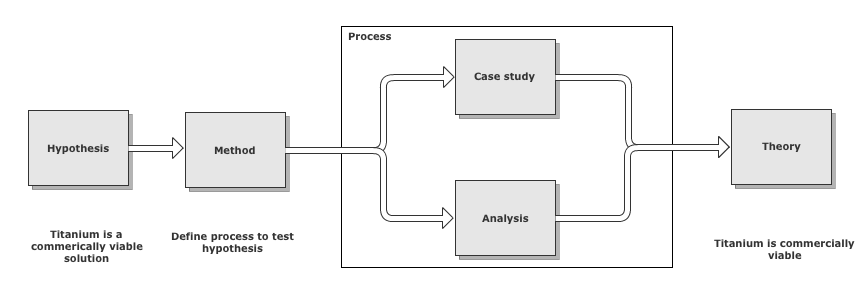
\includegraphics[scale=0.5]{images/process.png}\\{Main research process schematic}\\
\end{centering}

% summarize + go ahead for the next two chapters.
\paragraaf{Summary}
To answer whether or not the chosen solution is commercially viable a case study will be performed during which the solution will be analysed on provided criteria.